
\documentclass[12pt,oneside]{book}

\usepackage[a4paper,margin=1cm,nohead,foot=0.5cm]{geometry}
%\usepackage[legalpaper,margin=1cm,nohead,foot=0.5cm]{geometry}

\usepackage{graphicx}				% For adding images
\usepackage{float}					% For using float environments
\usepackage{booktabs}				% For table rules
\usepackage{times}					% For times font
\usepackage{lipsum}					% For generating random text

\usepackage{framed}
\usepackage{enumitem}


\usepackage{xcolor}         % colors
\usepackage{csvsimple}
\usepackage{amsmath,amssymb}
\usepackage{url}

\newcommand\sig[0]{\sigma}
\newcommand\act[1]{\phi_{#1}}

\newcommand\todo[1]{\textcolor{blue}{TODO: #1}}
\newcommand\edit[1]{{\color{blue} EDIT: }{\color{gray} #1}}

\pagestyle{plain}
\thispagestyle{empty}

\begin{document}

\begin{framed}
%\begin{minipage}{\textwidth}
\begin{center}
    \Huge \textbf{Inhibitor Gated RNNs -- Short Version}
\end{center}    
\Large
\noindent
\textbf{Motivation}: \begin{itemize}
    \item Quantized Gated RNNs that doesn't use Dot-product and Sigmoid.
\end{itemize}
%\vspace{0.2cm}

\noindent
\textbf{Basic idea}: 
%Let $u_t = W x_t + U h_{t-1} + b$ and change gated RNNs according to
%Take Manhattan distance $\left|Q_{ik} - K_{jk}\right|$ instead of Dot-prod, and  
\begin{itemize}
    \item Replace Dot-prod with Manhattan distance and Softmax with ReLU
\end{itemize}
\begin{equation*}
Q K^T \rightarrow \sum\nolimits_{k} \left|Q_{ik} - K_{jk}\right|
\end{equation*}
\begin{equation*}
\sum\nolimits_{j} \mathrm{Softmax} \left(Z_{ij}\right) V_{jk}  \rightarrow \sum_j \left( V_{jk} - Z_{ij}^+  \right)^+
    \label{eq:inhibition}
\end{equation*}
%such that multiplication is replaced with addition and sigmoid with ReLU.
%\vspace{0.1cm}
%
\noindent
\textbf{Observations}:
\begin{itemize}%[noitemsep]
    \item Reminiscent of subtractive inhibition in biological neurons.
    %\item The mechanism has similar limit behaviour as the conventional.
    \item Removes variable multiplication and require only \textit{half} precision.
    \item In the limits the modified gates behaves like the conventional.
\end{itemize}

\noindent
\textbf{Result}: 

\begin{itemize}
    \item Comparable training capacity to the conventional mechanism.
    \item Reduced precision requirements translate into computational efficiency.
    \item Substantional gains under FHE by avoiding ciphertext multiplication.
\end{itemize}

\noindent
\textbf{Potential}: 
\begin{itemize}
    \item Natural integer quantization for deployment under resource constraints.
    \item May enable end-to-end encrypted applications of Gated RNNs.
\end{itemize}

\noindent
\textbf{Future work}: 
\begin{itemize}
    \item Does this architecture generalize to transformers? Answer: Yes.
\end{itemize}

\iffalse
\begin{figure}[H]
    \centering
    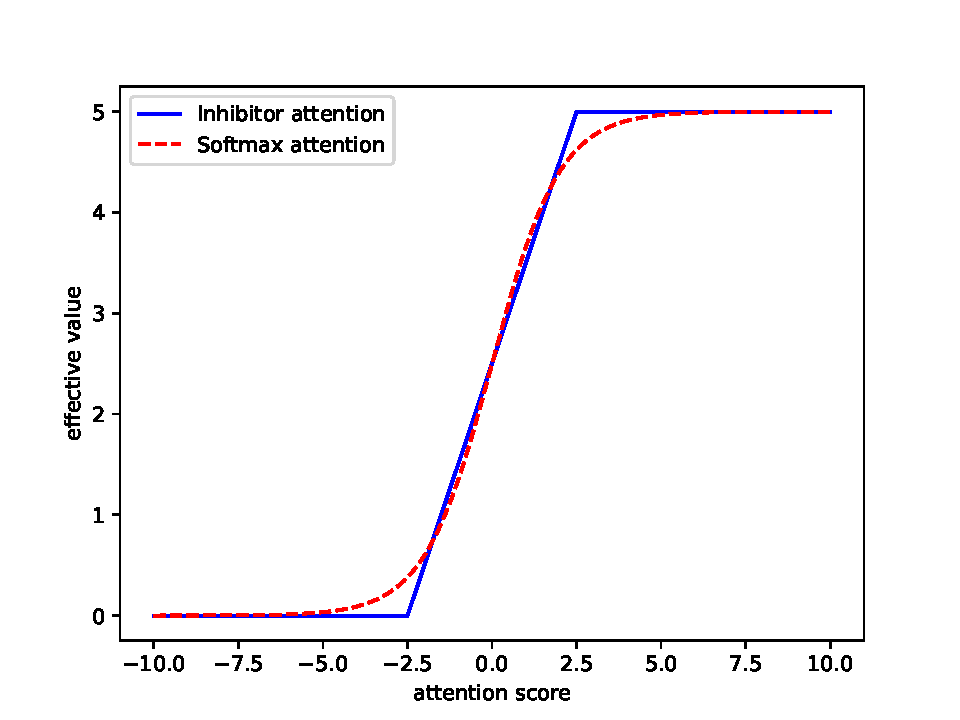
\includegraphics[width=0.8\columnwidth]{attention_comparison.pdf}
    %\caption{\large Comparison of the Inhibitor mechanism with conventional attention.}
    %\label{fig:figure1}
\end{figure}
\fi

%\end{minipage}
\end{framed}
 
\end{document}

